{
\usebackgroundtemplate{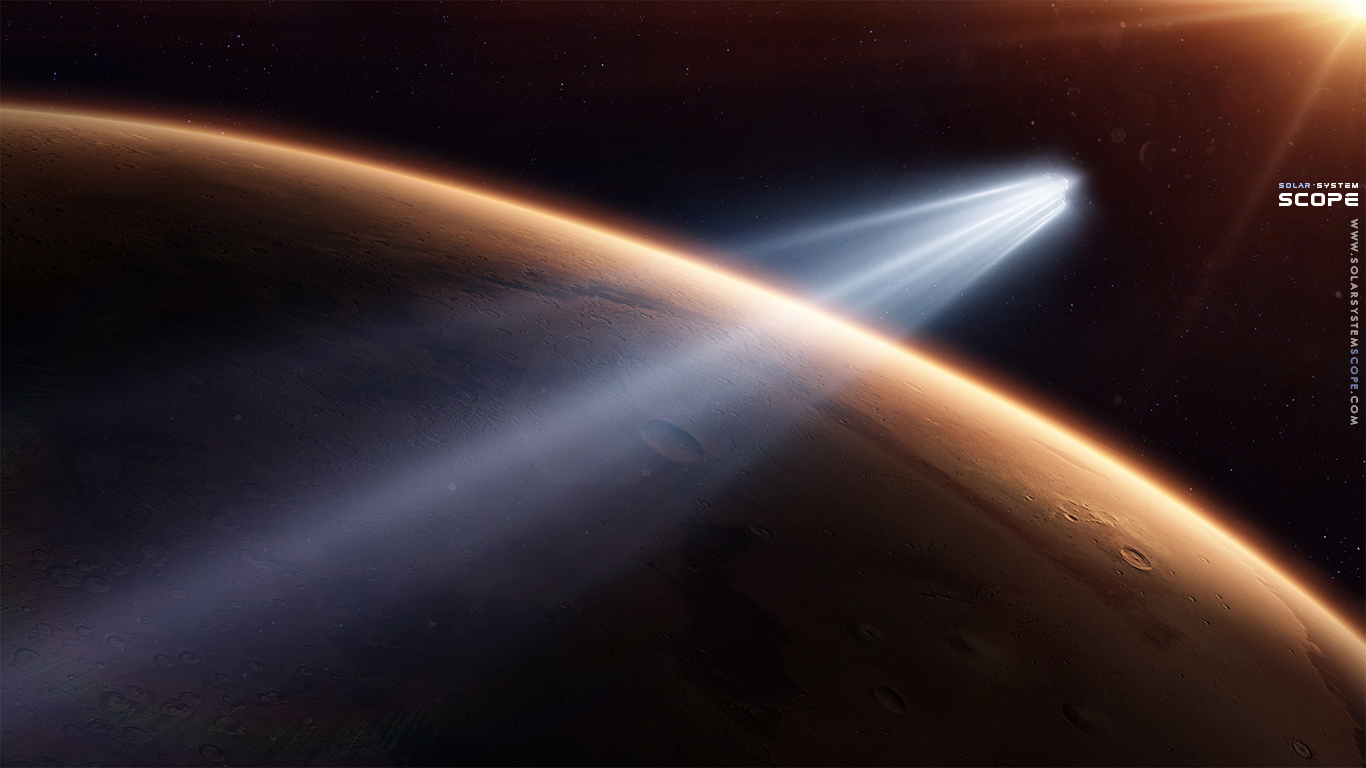
\includegraphics[height=\paperheight, keepaspectratio]{images/arive_at_target}}%
\begin{frame}
\end{frame}
\begin{frame}[t]{Sphere Of Influence}
    \begin{block}{}
    Sphere Of Influence(SOI) is the region around a planet in which the gravitational pull from the planet is bigger than
    any other body's gravitational pull. Which planet/body has the most gravitational influence on you
    \begin{itemize}
        \item We are in the SOI of the sun
        \item The moon is also influenced by the gravity of the sun
        \item but it is close enough to earth so that our gravitational influence is higher than the sun's
        \item therefor we say that the moon is within the SOI of earth
    \end{itemize}
    \end{block}
\end{frame}
\begin{frame}[t]{Intercept}
    \begin{block}{}
        When we are within the gravitational sphere of influence of the target planet we need to slow down to be
        captured by the planet.
        \begin{itemize}
            \item Burn retrograde to slow down
            \item Keep slowing down untill you fall into an highly eleptical orbit
            \item keep dropping periapsis to desired height
            \item wait for periapsis and then circularize orbit
        \end{itemize}
    \end{block}
\end{frame}
\begin{frame}[t]{Intercept}
    \begin{block}{Aerobreaking}
        Instead of having to circularize your orbit (which takes a fair amount of delta-v we can make use of the body's
        atmosphere to slow down to do this you need to
        \begin{itemize}
            \item drop periapsis just inside of the atmosphere
            \item not too deep because you can burn up
            \item not too shallow because slowing down would take a very long time
            \item just wait a couple of orbits
            \item the apoapsis should drop on every orbit because atmospheric drag slows you down while at periapsis
        \end{itemize}
    \end{block}
\end{frame}
}
\begin{frame}[t]{}
    \begin{block}{Aerobraking}
        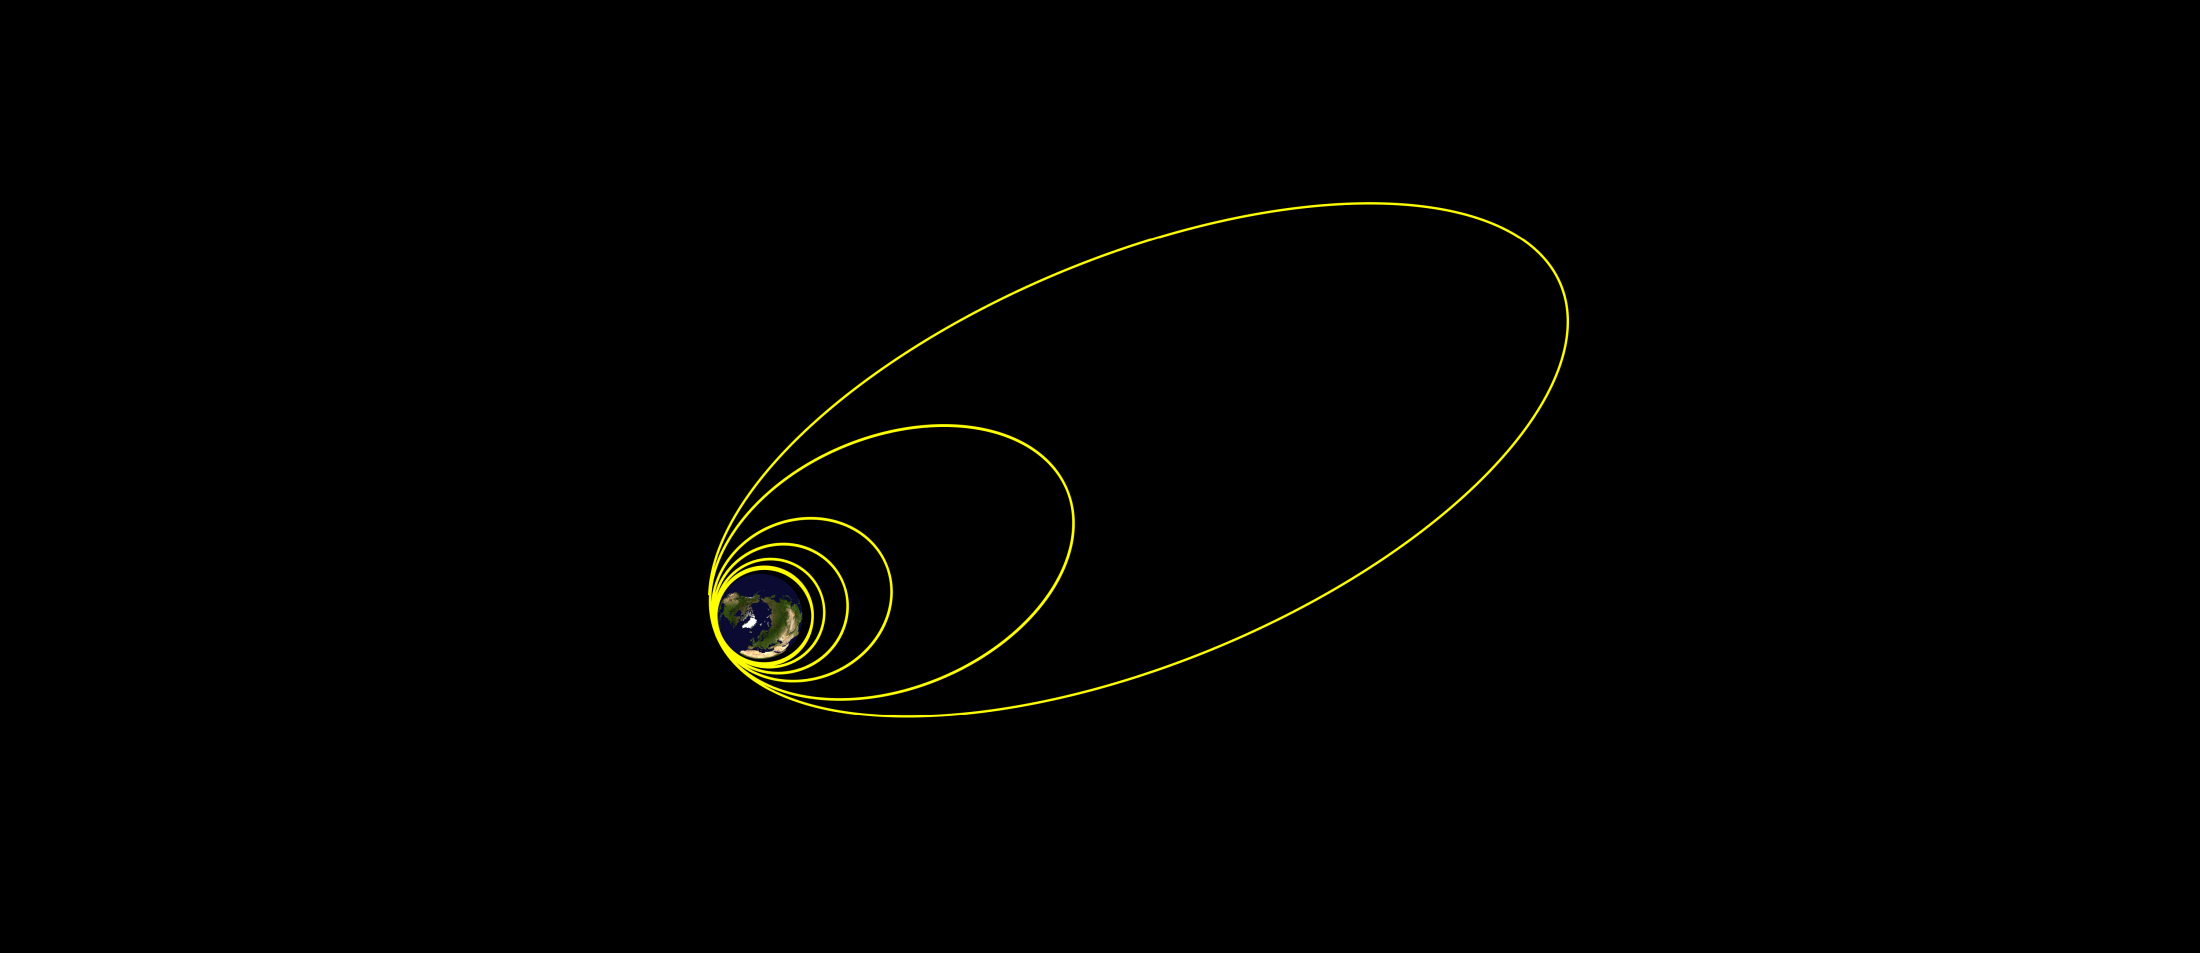
\includegraphics[width=\textwidth]{images/aerobraking}
    \end{block}
\end{frame}
